\documentclass[a4paper,10pt,warn]{article}
%\usepackage[T1]{fontenc}
%\usepackage[latin1]{inputenc}
%\usepackage{graphicx}
%\usepackage{float}
%\usepackage{amsmath}
%\usepackage{mathtools}

\usepackage{style}
\usepackage{float}
\usepackage{mcode}

\begin{document}
\title{Uppgift 1}
\author{Patrik Laurell, Bj�rn Wictorin}
\maketitle
\subsection*{a) Plottning av tabellv�rden}
\begin{figure}[h]
	\centering
	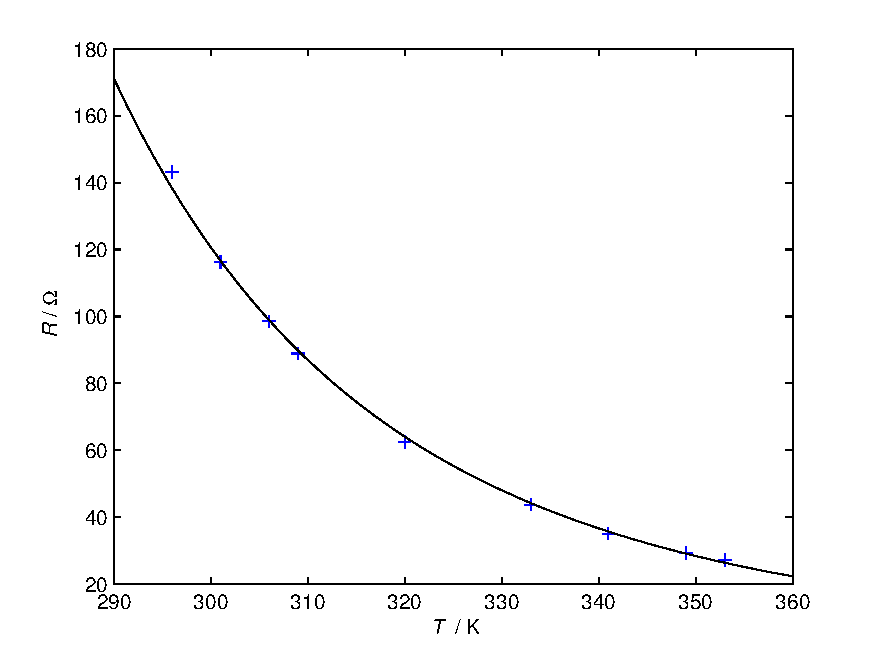
\includegraphics[width=0.8\textwidth]{../bilder/uppg1exp.pdf}
	\caption{Resistans som funktion av temperaturen.}
\end{figure}
Figur 1 visar resistansen f�r termistorn, som funktion av temperaturen. Korsen visar m�tv�rdena. Den svarta kurvan anpassades till datapunkterna med hj�lp av Matlab och ges av ekvationen $R=a\cdot e^{b/T}$, d�r $T$ �r terminstorns temperatur. 
	
\subsection*{b) Plottning av logaritmerade tabellv�rden}
Antag att sambandet kan skrivas $R = a \cdot e^{b/T}$. Logaritmering av h�ger- och v�nsterled ger $ln(R) = ln(a) + ln(e^{b/T}) = ln(a) + b\cdot \frac{1}{T}$. Detta �r ekvationen f�r en r�t linje, $y(1/T)$. Om v�rdena   $ln(R/\Omega)$ som funktion av $1/T$ ligger p� en r�t linje �r det allts� sannolikt att antagandet, $R = a \cdot e^{b/T}$, st�mmer. Figur 2 visar de logaritmerade resistansv�rdena som funktion av $1/T$, tillsammans med en anpassad r�t linje. I figuren ses att v�rdena ligger n�ra linjen, och allts� st�mmer modellen $R = a \cdot e^{b/T}$ bra med m�tdatan.
	
\begin{figure}
	\centering
	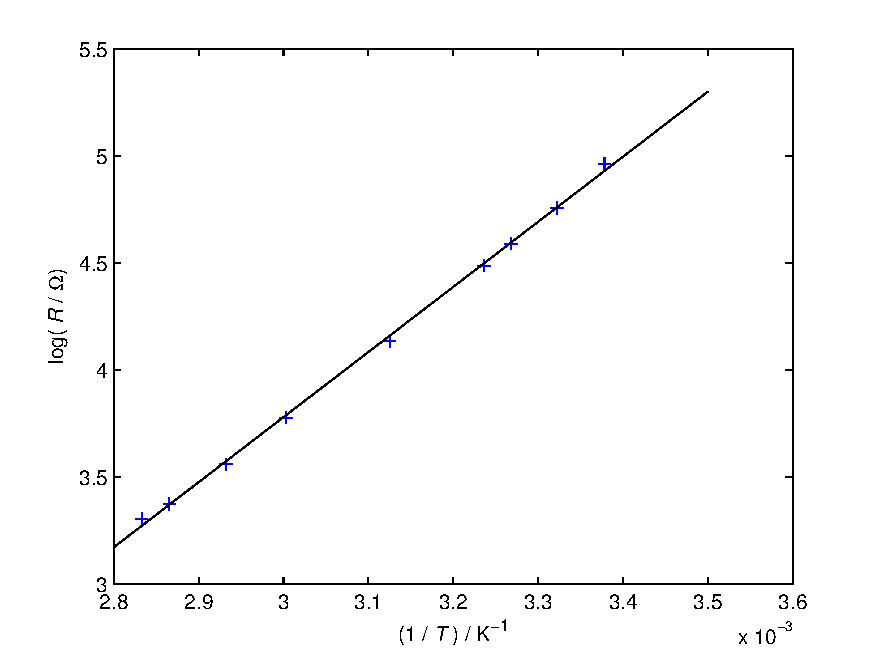
\includegraphics[width=0.8\textwidth]{../bilder/uppg1line.pdf}
	\caption{Logaritmerade m�tpunkter, $ln(R)$, som funktion av $1/T$.}
\end{figure}

\subsection*{c) R�tlinjeanpassning}
Som vi s�g i uppgift 1b ligger m�tpunkterna $ln(R)$ plottade mot $1/T$ n�ra en r�t linje. F�r att ta fram koefficienterna f�r linjen anv�ndes funktionen ``polyfit'' i Matlab. Det anpassade polynomet var av grad 1. Den anpassade linjen ges av ekvationen $y(1/T) = ln(a) + b \cdot \frac{1}{T}$. R�tlinjeanpassningen ger att $ln(a) = -5.34 \Leftrightarrow a=4.8 m\Omega$ och $b = 3040 K$.

\subsection*{d) Plottning av den r�ta linjen}
Den r�ta linjen plottades i samma figur som de logaritmerade m�tpunkterna, se figur 2.

\newpage
\section*{Matlab kod}
\lstinputlisting{../kod/inlamning1del1.m}

\end{document}